% Created by tikzDevice version 0.10.1 on 2018-05-18 21:51:37
% !TEX encoding = UTF-8 Unicode
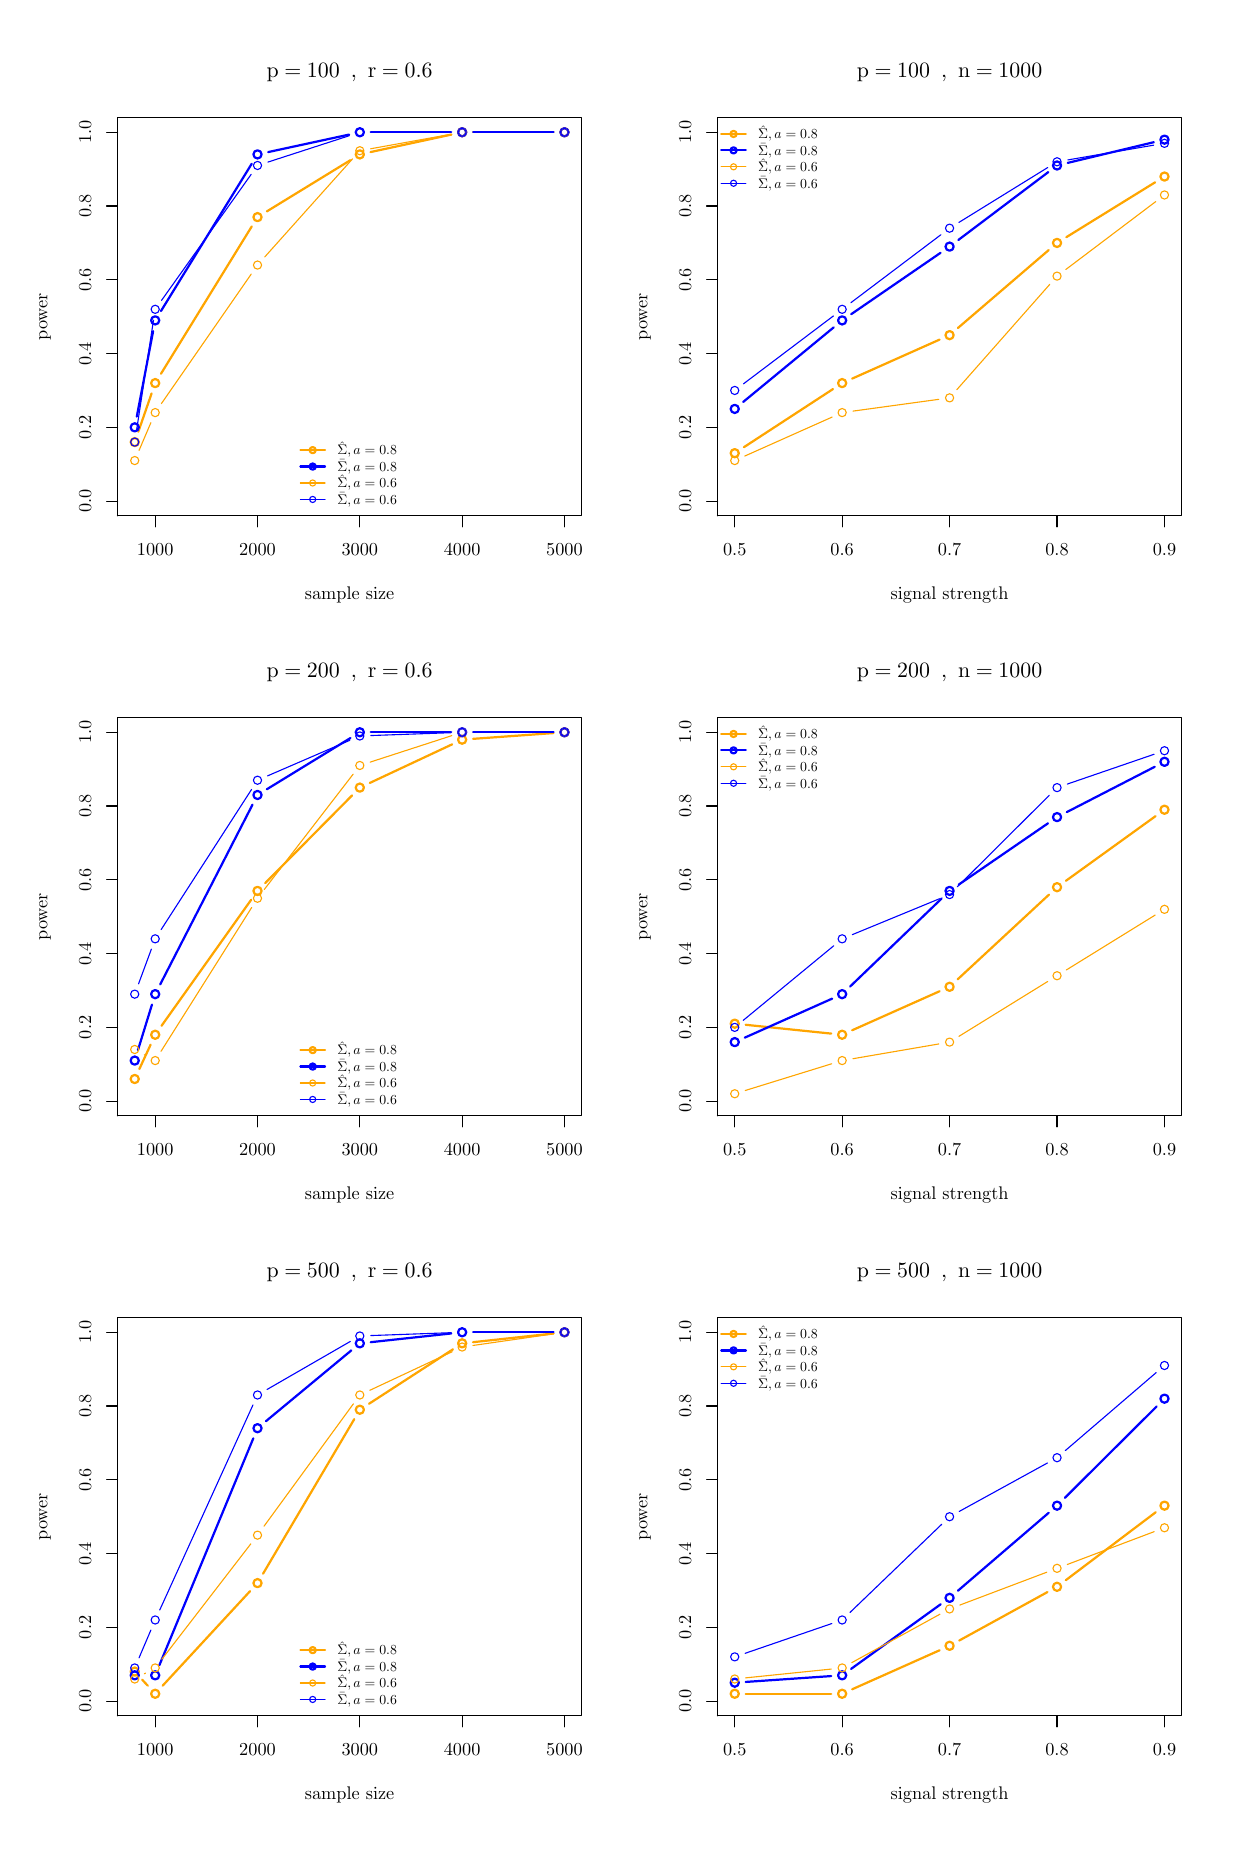
\begin{tikzpicture}[x=1pt,y=1pt]
\definecolor{fillColor}{RGB}{255,255,255}
\path[use as bounding box,fill=fillColor,fill opacity=0.00] (0,0) rectangle (433.62,650.43);
\begin{scope}
\path[clip] ( 32.47,474.01) rectangle (200.18,617.96);
\definecolor{drawColor}{RGB}{255,165,0}

\path[draw=drawColor,line width= 0.8pt,line join=round,line cap=round] ( 39.98,504.41) -- ( 44.78,518.25);

\path[draw=drawColor,line width= 0.8pt,line join=round,line cap=round] ( 48.16,525.36) -- ( 80.97,578.60);

\path[draw=drawColor,line width= 0.8pt,line join=round,line cap=round] ( 86.43,584.04) -- (116.65,602.56);

\path[draw=drawColor,line width= 0.8pt,line join=round,line cap=round] (123.89,605.47) -- (153.12,611.79);

\path[draw=drawColor,line width= 0.8pt,line join=round,line cap=round] (160.95,612.63) -- (190.01,612.63);

\path[draw=drawColor,line width= 0.8pt,line join=round,line cap=round] ( 38.68,500.67) circle (  1.48);

\path[draw=drawColor,line width= 0.8pt,line join=round,line cap=round] ( 46.08,521.99) circle (  1.48);

\path[draw=drawColor,line width= 0.8pt,line join=round,line cap=round] ( 83.05,581.97) circle (  1.48);

\path[draw=drawColor,line width= 0.8pt,line join=round,line cap=round] (120.02,604.63) circle (  1.48);

\path[draw=drawColor,line width= 0.8pt,line join=round,line cap=round] (156.99,612.63) circle (  1.48);

\path[draw=drawColor,line width= 0.8pt,line join=round,line cap=round] (193.97,612.63) circle (  1.48);
\end{scope}
\begin{scope}
\path[clip] (  0.00,  0.00) rectangle (433.62,650.43);
\definecolor{drawColor}{RGB}{0,0,0}

\path[draw=drawColor,line width= 0.4pt,line join=round,line cap=round] ( 46.08,474.01) -- (193.97,474.01);

\path[draw=drawColor,line width= 0.4pt,line join=round,line cap=round] ( 46.08,474.01) -- ( 46.08,470.05);

\path[draw=drawColor,line width= 0.4pt,line join=round,line cap=round] ( 83.05,474.01) -- ( 83.05,470.05);

\path[draw=drawColor,line width= 0.4pt,line join=round,line cap=round] (120.02,474.01) -- (120.02,470.05);

\path[draw=drawColor,line width= 0.4pt,line join=round,line cap=round] (156.99,474.01) -- (156.99,470.05);

\path[draw=drawColor,line width= 0.4pt,line join=round,line cap=round] (193.97,474.01) -- (193.97,470.05);

\node[text=drawColor,anchor=base,inner sep=0pt, outer sep=0pt, scale=  0.66] at ( 46.08,459.76) {1000};

\node[text=drawColor,anchor=base,inner sep=0pt, outer sep=0pt, scale=  0.66] at ( 83.05,459.76) {2000};

\node[text=drawColor,anchor=base,inner sep=0pt, outer sep=0pt, scale=  0.66] at (120.02,459.76) {3000};

\node[text=drawColor,anchor=base,inner sep=0pt, outer sep=0pt, scale=  0.66] at (156.99,459.76) {4000};

\node[text=drawColor,anchor=base,inner sep=0pt, outer sep=0pt, scale=  0.66] at (193.97,459.76) {5000};

\path[draw=drawColor,line width= 0.4pt,line join=round,line cap=round] ( 32.47,479.34) -- ( 32.47,612.63);

\path[draw=drawColor,line width= 0.4pt,line join=round,line cap=round] ( 32.47,479.34) -- ( 28.51,479.34);

\path[draw=drawColor,line width= 0.4pt,line join=round,line cap=round] ( 32.47,506.00) -- ( 28.51,506.00);

\path[draw=drawColor,line width= 0.4pt,line join=round,line cap=round] ( 32.47,532.66) -- ( 28.51,532.66);

\path[draw=drawColor,line width= 0.4pt,line join=round,line cap=round] ( 32.47,559.31) -- ( 28.51,559.31);

\path[draw=drawColor,line width= 0.4pt,line join=round,line cap=round] ( 32.47,585.97) -- ( 28.51,585.97);

\path[draw=drawColor,line width= 0.4pt,line join=round,line cap=round] ( 32.47,612.63) -- ( 28.51,612.63);

\node[text=drawColor,rotate= 90.00,anchor=base,inner sep=0pt, outer sep=0pt, scale=  0.66] at ( 22.97,479.34) {0.0};

\node[text=drawColor,rotate= 90.00,anchor=base,inner sep=0pt, outer sep=0pt, scale=  0.66] at ( 22.97,506.00) {0.2};

\node[text=drawColor,rotate= 90.00,anchor=base,inner sep=0pt, outer sep=0pt, scale=  0.66] at ( 22.97,532.66) {0.4};

\node[text=drawColor,rotate= 90.00,anchor=base,inner sep=0pt, outer sep=0pt, scale=  0.66] at ( 22.97,559.31) {0.6};

\node[text=drawColor,rotate= 90.00,anchor=base,inner sep=0pt, outer sep=0pt, scale=  0.66] at ( 22.97,585.97) {0.8};

\node[text=drawColor,rotate= 90.00,anchor=base,inner sep=0pt, outer sep=0pt, scale=  0.66] at ( 22.97,612.63) {1.0};

\path[draw=drawColor,line width= 0.4pt,line join=round,line cap=round] ( 32.47,474.01) --
	(200.18,474.01) --
	(200.18,617.96) --
	( 32.47,617.96) --
	( 32.47,474.01);
\end{scope}
\begin{scope}
\path[clip] (  0.00,433.62) rectangle (216.81,650.43);
\definecolor{drawColor}{RGB}{0,0,0}

\node[text=drawColor,anchor=base west,inner sep=0pt, outer sep=0pt, scale=  0.79] at ( 86.33,632.42) {p};

\node[text=drawColor,anchor=base west,inner sep=0pt, outer sep=0pt, scale=  0.79] at ( 92.74,632.42) {=};

\node[text=drawColor,anchor=base west,inner sep=0pt, outer sep=0pt, scale=  0.79] at (100.92,632.42) {100};

\node[text=drawColor,anchor=base west,inner sep=0pt, outer sep=0pt, scale=  0.79] at (112.79,632.42) { };

\node[text=drawColor,anchor=base west,inner sep=0pt, outer sep=0pt, scale=  0.79] at (116.75,632.42) {,};

\node[text=drawColor,anchor=base west,inner sep=0pt, outer sep=0pt, scale=  0.79] at (118.95,632.42) { };

\node[text=drawColor,anchor=base west,inner sep=0pt, outer sep=0pt, scale=  0.79] at (122.91,632.42) {r};

\node[text=drawColor,anchor=base west,inner sep=0pt, outer sep=0pt, scale=  0.79] at (128.03,632.42) {=};

\node[text=drawColor,anchor=base west,inner sep=0pt, outer sep=0pt, scale=  0.79] at (136.20,632.42) {0.6};

\node[text=drawColor,anchor=base,inner sep=0pt, outer sep=0pt, scale=  0.66] at (116.33,443.92) {sample size};

\node[text=drawColor,rotate= 90.00,anchor=base,inner sep=0pt, outer sep=0pt, scale=  0.66] at (  7.13,545.98) {power};
\end{scope}
\begin{scope}
\path[clip] ( 32.47,474.01) rectangle (200.18,617.96);
\definecolor{drawColor}{RGB}{0,0,255}

\path[draw=drawColor,line width= 0.8pt,line join=round,line cap=round] ( 39.43,509.89) -- ( 45.33,540.76);

\path[draw=drawColor,line width= 0.8pt,line join=round,line cap=round] ( 48.16,548.02) -- ( 80.97,601.26);

\path[draw=drawColor,line width= 0.8pt,line join=round,line cap=round] ( 86.92,605.47) -- (116.15,611.79);

\path[draw=drawColor,line width= 0.8pt,line join=round,line cap=round] (123.98,612.63) -- (153.03,612.63);

\path[draw=drawColor,line width= 0.8pt,line join=round,line cap=round] (160.95,612.63) -- (190.01,612.63);

\path[draw=drawColor,line width= 0.8pt,line join=round,line cap=round] ( 38.68,506.00) circle (  1.48);

\path[draw=drawColor,line width= 0.8pt,line join=round,line cap=round] ( 46.08,544.65) circle (  1.48);

\path[draw=drawColor,line width= 0.8pt,line join=round,line cap=round] ( 83.05,604.63) circle (  1.48);

\path[draw=drawColor,line width= 0.8pt,line join=round,line cap=round] (120.02,612.63) circle (  1.48);

\path[draw=drawColor,line width= 0.8pt,line join=round,line cap=round] (156.99,612.63) circle (  1.48);

\path[draw=drawColor,line width= 0.8pt,line join=round,line cap=round] (193.97,612.63) circle (  1.48);
\definecolor{drawColor}{RGB}{255,165,0}

\path[draw=drawColor,line width= 0.4pt,line join=round,line cap=round] ( 40.24,497.65) -- ( 44.52,507.69);

\path[draw=drawColor,line width= 0.4pt,line join=round,line cap=round] ( 48.33,514.59) -- ( 80.79,561.39);

\path[draw=drawColor,line width= 0.4pt,line join=round,line cap=round] ( 85.69,567.60) -- (117.38,603.01);

\path[draw=drawColor,line width= 0.4pt,line join=round,line cap=round] (123.92,606.66) -- (153.10,611.92);

\path[draw=drawColor,line width= 0.4pt,line join=round,line cap=round] (160.95,612.63) -- (190.01,612.63);

\path[draw=drawColor,line width= 0.4pt,line join=round,line cap=round] ( 38.68,494.00) circle (  1.48);

\path[draw=drawColor,line width= 0.4pt,line join=round,line cap=round] ( 46.08,511.33) circle (  1.48);

\path[draw=drawColor,line width= 0.4pt,line join=round,line cap=round] ( 83.05,564.64) circle (  1.48);

\path[draw=drawColor,line width= 0.4pt,line join=round,line cap=round] (120.02,605.96) circle (  1.48);

\path[draw=drawColor,line width= 0.4pt,line join=round,line cap=round] (156.99,612.63) circle (  1.48);

\path[draw=drawColor,line width= 0.4pt,line join=round,line cap=round] (193.97,612.63) circle (  1.48);
\definecolor{drawColor}{RGB}{0,0,255}

\path[draw=drawColor,line width= 0.4pt,line join=round,line cap=round] ( 39.29,504.58) -- ( 45.47,544.74);

\path[draw=drawColor,line width= 0.4pt,line join=round,line cap=round] ( 48.37,551.88) -- ( 80.75,597.40);

\path[draw=drawColor,line width= 0.4pt,line join=round,line cap=round] ( 86.82,601.85) -- (116.26,611.40);

\path[draw=drawColor,line width= 0.4pt,line join=round,line cap=round] (123.98,612.63) -- (153.03,612.63);

\path[draw=drawColor,line width= 0.4pt,line join=round,line cap=round] (160.95,612.63) -- (190.01,612.63);

\path[draw=drawColor,line width= 0.4pt,line join=round,line cap=round] ( 38.68,500.67) circle (  1.48);

\path[draw=drawColor,line width= 0.4pt,line join=round,line cap=round] ( 46.08,548.65) circle (  1.48);

\path[draw=drawColor,line width= 0.4pt,line join=round,line cap=round] ( 83.05,600.63) circle (  1.48);

\path[draw=drawColor,line width= 0.4pt,line join=round,line cap=round] (120.02,612.63) circle (  1.48);

\path[draw=drawColor,line width= 0.4pt,line join=round,line cap=round] (156.99,612.63) circle (  1.48);

\path[draw=drawColor,line width= 0.4pt,line join=round,line cap=round] (193.97,612.63) circle (  1.48);
\definecolor{drawColor}{RGB}{255,165,0}

\path[draw=drawColor,line width= 0.8pt,line join=round,line cap=round] ( 98.54,497.77) -- (107.45,497.77);
\definecolor{drawColor}{RGB}{0,0,255}

\path[draw=drawColor,line width= 0.8pt,line join=round,line cap=round] ( 98.54,491.83) -- (107.45,491.83);
\definecolor{drawColor}{RGB}{255,165,0}

\path[draw=drawColor,line width= 0.4pt,line join=round,line cap=round] ( 98.54,485.89) -- (107.45,485.89);
\definecolor{drawColor}{RGB}{0,0,255}

\path[draw=drawColor,line width= 0.4pt,line join=round,line cap=round] ( 98.54,479.95) -- (107.45,479.95);
\definecolor{drawColor}{RGB}{255,165,0}

\path[draw=drawColor,line width= 0.8pt,line join=round,line cap=round] (102.99,497.77) circle (  1.11);
\definecolor{drawColor}{RGB}{0,0,255}

\path[draw=drawColor,line width= 0.8pt,line join=round,line cap=round] (102.99,491.83) circle (  1.11);
\definecolor{drawColor}{RGB}{255,165,0}

\path[draw=drawColor,line width= 0.4pt,line join=round,line cap=round] (102.99,485.89) circle (  1.11);
\definecolor{drawColor}{RGB}{0,0,255}

\path[draw=drawColor,line width= 0.4pt,line join=round,line cap=round] (102.99,479.95) circle (  1.11);
\definecolor{drawColor}{RGB}{0,0,0}

\node[text=drawColor,anchor=base west,inner sep=0pt, outer sep=0pt, scale=  0.50] at (111.90,496.07) {$\hat{\Sigma},a=0.8$};

\node[text=drawColor,anchor=base west,inner sep=0pt, outer sep=0pt, scale=  0.50] at (111.90,490.13) {$\bar{\Sigma},a=0.8$};

\node[text=drawColor,anchor=base west,inner sep=0pt, outer sep=0pt, scale=  0.50] at (111.90,484.19) {$\hat{\Sigma},a=0.6$};

\node[text=drawColor,anchor=base west,inner sep=0pt, outer sep=0pt, scale=  0.50] at (111.90,478.25) {$\bar{\Sigma},a=0.6$};
\end{scope}
\begin{scope}
\path[clip] (249.28,474.01) rectangle (416.99,617.96);
\definecolor{drawColor}{RGB}{255,165,0}

\path[draw=drawColor,line width= 0.8pt,line join=round,line cap=round] (258.81,498.83) -- (291.00,519.83);

\path[draw=drawColor,line width= 0.8pt,line join=round,line cap=round] (297.93,523.61) -- (329.52,537.71);

\path[draw=drawColor,line width= 0.8pt,line join=round,line cap=round] (336.14,541.90) -- (368.95,570.06);

\path[draw=drawColor,line width= 0.8pt,line join=round,line cap=round] (375.32,574.72) -- (407.41,594.55);

\path[draw=drawColor,line width= 0.8pt,line join=round,line cap=round] (255.49,496.67) circle (  1.48);

\path[draw=drawColor,line width= 0.8pt,line join=round,line cap=round] (294.31,521.99) circle (  1.48);

\path[draw=drawColor,line width= 0.8pt,line join=round,line cap=round] (333.13,539.32) circle (  1.48);

\path[draw=drawColor,line width= 0.8pt,line join=round,line cap=round] (371.96,572.64) circle (  1.48);

\path[draw=drawColor,line width= 0.8pt,line join=round,line cap=round] (410.78,596.63) circle (  1.48);
\end{scope}
\begin{scope}
\path[clip] (  0.00,  0.00) rectangle (433.62,650.43);
\definecolor{drawColor}{RGB}{0,0,0}

\path[draw=drawColor,line width= 0.4pt,line join=round,line cap=round] (255.49,474.01) -- (410.78,474.01);

\path[draw=drawColor,line width= 0.4pt,line join=round,line cap=round] (255.49,474.01) -- (255.49,470.05);

\path[draw=drawColor,line width= 0.4pt,line join=round,line cap=round] (294.31,474.01) -- (294.31,470.05);

\path[draw=drawColor,line width= 0.4pt,line join=round,line cap=round] (333.14,474.01) -- (333.14,470.05);

\path[draw=drawColor,line width= 0.4pt,line join=round,line cap=round] (371.96,474.01) -- (371.96,470.05);

\path[draw=drawColor,line width= 0.4pt,line join=round,line cap=round] (410.78,474.01) -- (410.78,470.05);

\node[text=drawColor,anchor=base,inner sep=0pt, outer sep=0pt, scale=  0.66] at (255.49,459.76) {0.5};

\node[text=drawColor,anchor=base,inner sep=0pt, outer sep=0pt, scale=  0.66] at (294.31,459.76) {0.6};

\node[text=drawColor,anchor=base,inner sep=0pt, outer sep=0pt, scale=  0.66] at (333.14,459.76) {0.7};

\node[text=drawColor,anchor=base,inner sep=0pt, outer sep=0pt, scale=  0.66] at (371.96,459.76) {0.8};

\node[text=drawColor,anchor=base,inner sep=0pt, outer sep=0pt, scale=  0.66] at (410.78,459.76) {0.9};

\path[draw=drawColor,line width= 0.4pt,line join=round,line cap=round] (249.28,479.34) -- (249.28,612.63);

\path[draw=drawColor,line width= 0.4pt,line join=round,line cap=round] (249.28,479.34) -- (245.32,479.34);

\path[draw=drawColor,line width= 0.4pt,line join=round,line cap=round] (249.28,506.00) -- (245.32,506.00);

\path[draw=drawColor,line width= 0.4pt,line join=round,line cap=round] (249.28,532.66) -- (245.32,532.66);

\path[draw=drawColor,line width= 0.4pt,line join=round,line cap=round] (249.28,559.31) -- (245.32,559.31);

\path[draw=drawColor,line width= 0.4pt,line join=round,line cap=round] (249.28,585.97) -- (245.32,585.97);

\path[draw=drawColor,line width= 0.4pt,line join=round,line cap=round] (249.28,612.63) -- (245.32,612.63);

\node[text=drawColor,rotate= 90.00,anchor=base,inner sep=0pt, outer sep=0pt, scale=  0.66] at (239.78,479.34) {0.0};

\node[text=drawColor,rotate= 90.00,anchor=base,inner sep=0pt, outer sep=0pt, scale=  0.66] at (239.78,506.00) {0.2};

\node[text=drawColor,rotate= 90.00,anchor=base,inner sep=0pt, outer sep=0pt, scale=  0.66] at (239.78,532.66) {0.4};

\node[text=drawColor,rotate= 90.00,anchor=base,inner sep=0pt, outer sep=0pt, scale=  0.66] at (239.78,559.31) {0.6};

\node[text=drawColor,rotate= 90.00,anchor=base,inner sep=0pt, outer sep=0pt, scale=  0.66] at (239.78,585.97) {0.8};

\node[text=drawColor,rotate= 90.00,anchor=base,inner sep=0pt, outer sep=0pt, scale=  0.66] at (239.78,612.63) {1.0};

\path[draw=drawColor,line width= 0.4pt,line join=round,line cap=round] (249.28,474.01) --
	(416.99,474.01) --
	(416.99,617.96) --
	(249.28,617.96) --
	(249.28,474.01);
\end{scope}
\begin{scope}
\path[clip] (216.81,433.62) rectangle (433.62,650.43);
\definecolor{drawColor}{RGB}{0,0,0}

\node[text=drawColor,anchor=base west,inner sep=0pt, outer sep=0pt, scale=  0.79] at (299.63,632.42) {p};

\node[text=drawColor,anchor=base west,inner sep=0pt, outer sep=0pt, scale=  0.79] at (306.04,632.42) {=};

\node[text=drawColor,anchor=base west,inner sep=0pt, outer sep=0pt, scale=  0.79] at (314.22,632.42) {100};

\node[text=drawColor,anchor=base west,inner sep=0pt, outer sep=0pt, scale=  0.79] at (326.10,632.42) { };

\node[text=drawColor,anchor=base west,inner sep=0pt, outer sep=0pt, scale=  0.79] at (330.06,632.42) {,};

\node[text=drawColor,anchor=base west,inner sep=0pt, outer sep=0pt, scale=  0.79] at (332.26,632.42) { };

\node[text=drawColor,anchor=base west,inner sep=0pt, outer sep=0pt, scale=  0.79] at (336.21,632.42) {n};

\node[text=drawColor,anchor=base west,inner sep=0pt, outer sep=0pt, scale=  0.79] at (342.63,632.42) {=};

\node[text=drawColor,anchor=base west,inner sep=0pt, outer sep=0pt, scale=  0.79] at (350.80,632.42) {1000};

\node[text=drawColor,anchor=base,inner sep=0pt, outer sep=0pt, scale=  0.66] at (333.13,443.92) {signal strength};

\node[text=drawColor,rotate= 90.00,anchor=base,inner sep=0pt, outer sep=0pt, scale=  0.66] at (223.94,545.98) {power};
\end{scope}
\begin{scope}
\path[clip] (249.28,474.01) rectangle (416.99,617.96);
\definecolor{drawColor}{RGB}{0,0,255}

\path[draw=drawColor,line width= 0.8pt,line join=round,line cap=round] (258.55,515.18) -- (291.26,542.13);

\path[draw=drawColor,line width= 0.8pt,line join=round,line cap=round] (297.58,546.89) -- (329.87,569.07);

\path[draw=drawColor,line width= 0.8pt,line join=round,line cap=round] (336.29,573.70) -- (368.80,598.24);

\path[draw=drawColor,line width= 0.8pt,line join=round,line cap=round] (375.81,601.56) -- (406.93,609.04);

\path[draw=drawColor,line width= 0.8pt,line join=round,line cap=round] (255.49,512.66) circle (  1.48);

\path[draw=drawColor,line width= 0.8pt,line join=round,line cap=round] (294.31,544.65) circle (  1.48);

\path[draw=drawColor,line width= 0.8pt,line join=round,line cap=round] (333.13,571.31) circle (  1.48);

\path[draw=drawColor,line width= 0.8pt,line join=round,line cap=round] (371.96,600.63) circle (  1.48);

\path[draw=drawColor,line width= 0.8pt,line join=round,line cap=round] (410.78,609.96) circle (  1.48);
\definecolor{drawColor}{RGB}{255,165,0}

\path[draw=drawColor,line width= 0.4pt,line join=round,line cap=round] (259.11,495.62) -- (290.70,509.72);

\path[draw=drawColor,line width= 0.4pt,line join=round,line cap=round] (298.24,511.87) -- (329.21,516.12);

\path[draw=drawColor,line width= 0.4pt,line join=round,line cap=round] (335.76,519.63) -- (369.34,557.68);

\path[draw=drawColor,line width= 0.4pt,line join=round,line cap=round] (375.12,563.03) -- (407.62,587.58);

\path[draw=drawColor,line width= 0.4pt,line join=round,line cap=round] (255.49,494.00) circle (  1.48);

\path[draw=drawColor,line width= 0.4pt,line join=round,line cap=round] (294.31,511.33) circle (  1.48);

\path[draw=drawColor,line width= 0.4pt,line join=round,line cap=round] (333.13,516.66) circle (  1.48);

\path[draw=drawColor,line width= 0.4pt,line join=round,line cap=round] (371.96,560.65) circle (  1.48);

\path[draw=drawColor,line width= 0.4pt,line join=round,line cap=round] (410.78,589.97) circle (  1.48);
\definecolor{drawColor}{RGB}{0,0,255}

\path[draw=drawColor,line width= 0.4pt,line join=round,line cap=round] (258.65,521.72) -- (291.15,546.26);

\path[draw=drawColor,line width= 0.4pt,line join=round,line cap=round] (297.47,551.04) -- (329.98,575.59);

\path[draw=drawColor,line width= 0.4pt,line join=round,line cap=round] (336.50,580.05) -- (368.59,599.88);

\path[draw=drawColor,line width= 0.4pt,line join=round,line cap=round] (375.86,602.63) -- (406.87,607.96);

\path[draw=drawColor,line width= 0.4pt,line join=round,line cap=round] (255.49,519.33) circle (  1.48);

\path[draw=drawColor,line width= 0.4pt,line join=round,line cap=round] (294.31,548.65) circle (  1.48);

\path[draw=drawColor,line width= 0.4pt,line join=round,line cap=round] (333.13,577.97) circle (  1.48);

\path[draw=drawColor,line width= 0.4pt,line join=round,line cap=round] (371.96,601.96) circle (  1.48);

\path[draw=drawColor,line width= 0.4pt,line join=round,line cap=round] (410.78,608.63) circle (  1.48);
\definecolor{drawColor}{RGB}{255,165,0}

\path[draw=drawColor,line width= 0.8pt,line join=round,line cap=round] (250.62,612.02) -- (259.53,612.02);
\definecolor{drawColor}{RGB}{0,0,255}

\path[draw=drawColor,line width= 0.8pt,line join=round,line cap=round] (250.62,606.08) -- (259.53,606.08);
\definecolor{drawColor}{RGB}{255,165,0}

\path[draw=drawColor,line width= 0.4pt,line join=round,line cap=round] (250.62,600.14) -- (259.53,600.14);
\definecolor{drawColor}{RGB}{0,0,255}

\path[draw=drawColor,line width= 0.4pt,line join=round,line cap=round] (250.62,594.20) -- (259.53,594.20);
\definecolor{drawColor}{RGB}{255,165,0}

\path[draw=drawColor,line width= 0.8pt,line join=round,line cap=round] (255.07,612.02) circle (  1.11);
\definecolor{drawColor}{RGB}{0,0,255}

\path[draw=drawColor,line width= 0.8pt,line join=round,line cap=round] (255.07,606.08) circle (  1.11);
\definecolor{drawColor}{RGB}{255,165,0}

\path[draw=drawColor,line width= 0.4pt,line join=round,line cap=round] (255.07,600.14) circle (  1.11);
\definecolor{drawColor}{RGB}{0,0,255}

\path[draw=drawColor,line width= 0.4pt,line join=round,line cap=round] (255.07,594.20) circle (  1.11);
\definecolor{drawColor}{RGB}{0,0,0}

\node[text=drawColor,anchor=base west,inner sep=0pt, outer sep=0pt, scale=  0.50] at (263.98,610.31) {$\hat{\Sigma},a=0.8$};

\node[text=drawColor,anchor=base west,inner sep=0pt, outer sep=0pt, scale=  0.50] at (263.98,604.37) {$\bar{\Sigma},a=0.8$};

\node[text=drawColor,anchor=base west,inner sep=0pt, outer sep=0pt, scale=  0.50] at (263.98,598.43) {$\hat{\Sigma},a=0.6$};

\node[text=drawColor,anchor=base west,inner sep=0pt, outer sep=0pt, scale=  0.50] at (263.98,592.49) {$\bar{\Sigma},a=0.6$};
\end{scope}
\begin{scope}
\path[clip] ( 32.47,257.20) rectangle (200.18,401.15);
\definecolor{drawColor}{RGB}{255,165,0}

\path[draw=drawColor,line width= 0.8pt,line join=round,line cap=round] ( 40.35,274.12) -- ( 44.42,282.93);

\path[draw=drawColor,line width= 0.8pt,line join=round,line cap=round] ( 48.37,289.75) -- ( 80.75,335.28);

\path[draw=drawColor,line width= 0.8pt,line join=round,line cap=round] ( 85.84,341.32) -- (117.24,373.01);

\path[draw=drawColor,line width= 0.8pt,line join=round,line cap=round] (123.61,377.50) -- (153.41,391.47);

\path[draw=drawColor,line width= 0.8pt,line join=round,line cap=round] (160.94,393.44) -- (190.02,395.53);

\path[draw=drawColor,line width= 0.8pt,line join=round,line cap=round] ( 38.68,270.53) circle (  1.48);

\path[draw=drawColor,line width= 0.8pt,line join=round,line cap=round] ( 46.08,286.52) circle (  1.48);

\path[draw=drawColor,line width= 0.8pt,line join=round,line cap=round] ( 83.05,338.50) circle (  1.48);

\path[draw=drawColor,line width= 0.8pt,line join=round,line cap=round] (120.02,375.82) circle (  1.48);

\path[draw=drawColor,line width= 0.8pt,line join=round,line cap=round] (156.99,393.15) circle (  1.48);

\path[draw=drawColor,line width= 0.8pt,line join=round,line cap=round] (193.97,395.82) circle (  1.48);
\end{scope}
\begin{scope}
\path[clip] (  0.00,  0.00) rectangle (433.62,650.43);
\definecolor{drawColor}{RGB}{0,0,0}

\path[draw=drawColor,line width= 0.4pt,line join=round,line cap=round] ( 46.08,257.20) -- (193.97,257.20);

\path[draw=drawColor,line width= 0.4pt,line join=round,line cap=round] ( 46.08,257.20) -- ( 46.08,253.24);

\path[draw=drawColor,line width= 0.4pt,line join=round,line cap=round] ( 83.05,257.20) -- ( 83.05,253.24);

\path[draw=drawColor,line width= 0.4pt,line join=round,line cap=round] (120.02,257.20) -- (120.02,253.24);

\path[draw=drawColor,line width= 0.4pt,line join=round,line cap=round] (156.99,257.20) -- (156.99,253.24);

\path[draw=drawColor,line width= 0.4pt,line join=round,line cap=round] (193.97,257.20) -- (193.97,253.24);

\node[text=drawColor,anchor=base,inner sep=0pt, outer sep=0pt, scale=  0.66] at ( 46.08,242.95) {1000};

\node[text=drawColor,anchor=base,inner sep=0pt, outer sep=0pt, scale=  0.66] at ( 83.05,242.95) {2000};

\node[text=drawColor,anchor=base,inner sep=0pt, outer sep=0pt, scale=  0.66] at (120.02,242.95) {3000};

\node[text=drawColor,anchor=base,inner sep=0pt, outer sep=0pt, scale=  0.66] at (156.99,242.95) {4000};

\node[text=drawColor,anchor=base,inner sep=0pt, outer sep=0pt, scale=  0.66] at (193.97,242.95) {5000};

\path[draw=drawColor,line width= 0.4pt,line join=round,line cap=round] ( 32.47,262.53) -- ( 32.47,395.82);

\path[draw=drawColor,line width= 0.4pt,line join=round,line cap=round] ( 32.47,262.53) -- ( 28.51,262.53);

\path[draw=drawColor,line width= 0.4pt,line join=round,line cap=round] ( 32.47,289.19) -- ( 28.51,289.19);

\path[draw=drawColor,line width= 0.4pt,line join=round,line cap=round] ( 32.47,315.85) -- ( 28.51,315.85);

\path[draw=drawColor,line width= 0.4pt,line join=round,line cap=round] ( 32.47,342.50) -- ( 28.51,342.50);

\path[draw=drawColor,line width= 0.4pt,line join=round,line cap=round] ( 32.47,369.16) -- ( 28.51,369.16);

\path[draw=drawColor,line width= 0.4pt,line join=round,line cap=round] ( 32.47,395.82) -- ( 28.51,395.82);

\node[text=drawColor,rotate= 90.00,anchor=base,inner sep=0pt, outer sep=0pt, scale=  0.66] at ( 22.97,262.53) {0.0};

\node[text=drawColor,rotate= 90.00,anchor=base,inner sep=0pt, outer sep=0pt, scale=  0.66] at ( 22.97,289.19) {0.2};

\node[text=drawColor,rotate= 90.00,anchor=base,inner sep=0pt, outer sep=0pt, scale=  0.66] at ( 22.97,315.85) {0.4};

\node[text=drawColor,rotate= 90.00,anchor=base,inner sep=0pt, outer sep=0pt, scale=  0.66] at ( 22.97,342.50) {0.6};

\node[text=drawColor,rotate= 90.00,anchor=base,inner sep=0pt, outer sep=0pt, scale=  0.66] at ( 22.97,369.16) {0.8};

\node[text=drawColor,rotate= 90.00,anchor=base,inner sep=0pt, outer sep=0pt, scale=  0.66] at ( 22.97,395.82) {1.0};

\path[draw=drawColor,line width= 0.4pt,line join=round,line cap=round] ( 32.47,257.20) --
	(200.18,257.20) --
	(200.18,401.15) --
	( 32.47,401.15) --
	( 32.47,257.20);
\end{scope}
\begin{scope}
\path[clip] (  0.00,216.81) rectangle (216.81,433.62);
\definecolor{drawColor}{RGB}{0,0,0}

\node[text=drawColor,anchor=base west,inner sep=0pt, outer sep=0pt, scale=  0.79] at ( 86.33,415.61) {p};

\node[text=drawColor,anchor=base west,inner sep=0pt, outer sep=0pt, scale=  0.79] at ( 92.74,415.61) {=};

\node[text=drawColor,anchor=base west,inner sep=0pt, outer sep=0pt, scale=  0.79] at (100.92,415.61) {200};

\node[text=drawColor,anchor=base west,inner sep=0pt, outer sep=0pt, scale=  0.79] at (112.79,415.61) { };

\node[text=drawColor,anchor=base west,inner sep=0pt, outer sep=0pt, scale=  0.79] at (116.75,415.61) {,};

\node[text=drawColor,anchor=base west,inner sep=0pt, outer sep=0pt, scale=  0.79] at (118.95,415.61) { };

\node[text=drawColor,anchor=base west,inner sep=0pt, outer sep=0pt, scale=  0.79] at (122.91,415.61) {r};

\node[text=drawColor,anchor=base west,inner sep=0pt, outer sep=0pt, scale=  0.79] at (128.03,415.61) {=};

\node[text=drawColor,anchor=base west,inner sep=0pt, outer sep=0pt, scale=  0.79] at (136.20,415.61) {0.6};

\node[text=drawColor,anchor=base,inner sep=0pt, outer sep=0pt, scale=  0.66] at (116.33,227.11) {sample size};

\node[text=drawColor,rotate= 90.00,anchor=base,inner sep=0pt, outer sep=0pt, scale=  0.66] at (  7.13,329.17) {power};
\end{scope}
\begin{scope}
\path[clip] ( 32.47,257.20) rectangle (200.18,401.15);
\definecolor{drawColor}{RGB}{0,0,255}

\path[draw=drawColor,line width= 0.8pt,line join=round,line cap=round] ( 39.85,280.98) -- ( 44.91,297.40);

\path[draw=drawColor,line width= 0.8pt,line join=round,line cap=round] ( 47.89,304.71) -- ( 81.24,369.64);

\path[draw=drawColor,line width= 0.8pt,line join=round,line cap=round] ( 86.43,375.23) -- (116.65,393.75);

\path[draw=drawColor,line width= 0.8pt,line join=round,line cap=round] (123.98,395.82) -- (153.03,395.82);

\path[draw=drawColor,line width= 0.8pt,line join=round,line cap=round] (160.95,395.82) -- (190.01,395.82);

\path[draw=drawColor,line width= 0.8pt,line join=round,line cap=round] ( 38.68,277.19) circle (  1.48);

\path[draw=drawColor,line width= 0.8pt,line join=round,line cap=round] ( 46.08,301.19) circle (  1.48);

\path[draw=drawColor,line width= 0.8pt,line join=round,line cap=round] ( 83.05,373.16) circle (  1.48);

\path[draw=drawColor,line width= 0.8pt,line join=round,line cap=round] (120.02,395.82) circle (  1.48);

\path[draw=drawColor,line width= 0.8pt,line join=round,line cap=round] (156.99,395.82) circle (  1.48);

\path[draw=drawColor,line width= 0.8pt,line join=round,line cap=round] (193.97,395.82) circle (  1.48);
\definecolor{drawColor}{RGB}{255,165,0}

\path[draw=drawColor,line width= 0.4pt,line join=round,line cap=round] ( 42.17,279.31) -- ( 42.59,279.08);

\path[draw=drawColor,line width= 0.4pt,line join=round,line cap=round] ( 48.19,280.54) -- ( 80.94,332.49);

\path[draw=drawColor,line width= 0.4pt,line join=round,line cap=round] ( 85.47,338.98) -- (117.61,380.68);

\path[draw=drawColor,line width= 0.4pt,line join=round,line cap=round] (123.79,385.04) -- (153.23,394.59);

\path[draw=drawColor,line width= 0.4pt,line join=round,line cap=round] (160.95,395.82) -- (190.01,395.82);

\path[draw=drawColor,line width= 0.4pt,line join=round,line cap=round] ( 38.68,281.19) circle (  1.48);

\path[draw=drawColor,line width= 0.4pt,line join=round,line cap=round] ( 46.08,277.19) circle (  1.48);

\path[draw=drawColor,line width= 0.4pt,line join=round,line cap=round] ( 83.05,335.84) circle (  1.48);

\path[draw=drawColor,line width= 0.4pt,line join=round,line cap=round] (120.02,383.82) circle (  1.48);

\path[draw=drawColor,line width= 0.4pt,line join=round,line cap=round] (156.99,395.82) circle (  1.48);

\path[draw=drawColor,line width= 0.4pt,line join=round,line cap=round] (193.97,395.82) circle (  1.48);
\definecolor{drawColor}{RGB}{0,0,255}

\path[draw=drawColor,line width= 0.4pt,line join=round,line cap=round] ( 40.06,304.90) -- ( 44.70,317.46);

\path[draw=drawColor,line width= 0.4pt,line join=round,line cap=round] ( 48.22,324.51) -- ( 80.90,375.16);

\path[draw=drawColor,line width= 0.4pt,line join=round,line cap=round] ( 86.68,380.06) -- (116.39,392.91);

\path[draw=drawColor,line width= 0.4pt,line join=round,line cap=round] (123.98,394.63) -- (153.04,395.67);

\path[draw=drawColor,line width= 0.4pt,line join=round,line cap=round] (160.95,395.82) -- (190.01,395.82);

\path[draw=drawColor,line width= 0.4pt,line join=round,line cap=round] ( 38.68,301.19) circle (  1.48);

\path[draw=drawColor,line width= 0.4pt,line join=round,line cap=round] ( 46.08,321.18) circle (  1.48);

\path[draw=drawColor,line width= 0.4pt,line join=round,line cap=round] ( 83.05,378.49) circle (  1.48);

\path[draw=drawColor,line width= 0.4pt,line join=round,line cap=round] (120.02,394.48) circle (  1.48);

\path[draw=drawColor,line width= 0.4pt,line join=round,line cap=round] (156.99,395.82) circle (  1.48);

\path[draw=drawColor,line width= 0.4pt,line join=round,line cap=round] (193.97,395.82) circle (  1.48);
\definecolor{drawColor}{RGB}{255,165,0}

\path[draw=drawColor,line width= 0.8pt,line join=round,line cap=round] ( 98.54,280.96) -- (107.45,280.96);
\definecolor{drawColor}{RGB}{0,0,255}

\path[draw=drawColor,line width= 0.8pt,line join=round,line cap=round] ( 98.54,275.02) -- (107.45,275.02);
\definecolor{drawColor}{RGB}{255,165,0}

\path[draw=drawColor,line width= 0.4pt,line join=round,line cap=round] ( 98.54,269.08) -- (107.45,269.08);
\definecolor{drawColor}{RGB}{0,0,255}

\path[draw=drawColor,line width= 0.4pt,line join=round,line cap=round] ( 98.54,263.14) -- (107.45,263.14);
\definecolor{drawColor}{RGB}{255,165,0}

\path[draw=drawColor,line width= 0.8pt,line join=round,line cap=round] (102.99,280.96) circle (  1.11);
\definecolor{drawColor}{RGB}{0,0,255}

\path[draw=drawColor,line width= 0.8pt,line join=round,line cap=round] (102.99,275.02) circle (  1.11);
\definecolor{drawColor}{RGB}{255,165,0}

\path[draw=drawColor,line width= 0.4pt,line join=round,line cap=round] (102.99,269.08) circle (  1.11);
\definecolor{drawColor}{RGB}{0,0,255}

\path[draw=drawColor,line width= 0.4pt,line join=round,line cap=round] (102.99,263.14) circle (  1.11);
\definecolor{drawColor}{RGB}{0,0,0}

\node[text=drawColor,anchor=base west,inner sep=0pt, outer sep=0pt, scale=  0.50] at (111.90,279.26) {$\hat{\Sigma},a=0.8$};

\node[text=drawColor,anchor=base west,inner sep=0pt, outer sep=0pt, scale=  0.50] at (111.90,273.32) {$\bar{\Sigma},a=0.8$};

\node[text=drawColor,anchor=base west,inner sep=0pt, outer sep=0pt, scale=  0.50] at (111.90,267.38) {$\hat{\Sigma},a=0.6$};

\node[text=drawColor,anchor=base west,inner sep=0pt, outer sep=0pt, scale=  0.50] at (111.90,261.44) {$\bar{\Sigma},a=0.6$};
\end{scope}
\begin{scope}
\path[clip] (249.28,257.20) rectangle (416.99,401.15);
\definecolor{drawColor}{RGB}{255,165,0}

\path[draw=drawColor,line width= 0.8pt,line join=round,line cap=round] (259.43,290.12) -- (290.38,286.93);

\path[draw=drawColor,line width= 0.8pt,line join=round,line cap=round] (297.93,288.14) -- (329.52,302.24);

\path[draw=drawColor,line width= 0.8pt,line join=round,line cap=round] (336.04,306.54) -- (369.05,337.15);

\path[draw=drawColor,line width= 0.8pt,line join=round,line cap=round] (375.17,342.15) -- (407.56,365.51);

\path[draw=drawColor,line width= 0.8pt,line join=round,line cap=round] (255.49,290.52) circle (  1.48);

\path[draw=drawColor,line width= 0.8pt,line join=round,line cap=round] (294.31,286.52) circle (  1.48);

\path[draw=drawColor,line width= 0.8pt,line join=round,line cap=round] (333.13,303.85) circle (  1.48);

\path[draw=drawColor,line width= 0.8pt,line join=round,line cap=round] (371.96,339.84) circle (  1.48);

\path[draw=drawColor,line width= 0.8pt,line join=round,line cap=round] (410.78,367.83) circle (  1.48);
\end{scope}
\begin{scope}
\path[clip] (  0.00,  0.00) rectangle (433.62,650.43);
\definecolor{drawColor}{RGB}{0,0,0}

\path[draw=drawColor,line width= 0.4pt,line join=round,line cap=round] (255.49,257.20) -- (410.78,257.20);

\path[draw=drawColor,line width= 0.4pt,line join=round,line cap=round] (255.49,257.20) -- (255.49,253.24);

\path[draw=drawColor,line width= 0.4pt,line join=round,line cap=round] (294.31,257.20) -- (294.31,253.24);

\path[draw=drawColor,line width= 0.4pt,line join=round,line cap=round] (333.14,257.20) -- (333.14,253.24);

\path[draw=drawColor,line width= 0.4pt,line join=round,line cap=round] (371.96,257.20) -- (371.96,253.24);

\path[draw=drawColor,line width= 0.4pt,line join=round,line cap=round] (410.78,257.20) -- (410.78,253.24);

\node[text=drawColor,anchor=base,inner sep=0pt, outer sep=0pt, scale=  0.66] at (255.49,242.95) {0.5};

\node[text=drawColor,anchor=base,inner sep=0pt, outer sep=0pt, scale=  0.66] at (294.31,242.95) {0.6};

\node[text=drawColor,anchor=base,inner sep=0pt, outer sep=0pt, scale=  0.66] at (333.14,242.95) {0.7};

\node[text=drawColor,anchor=base,inner sep=0pt, outer sep=0pt, scale=  0.66] at (371.96,242.95) {0.8};

\node[text=drawColor,anchor=base,inner sep=0pt, outer sep=0pt, scale=  0.66] at (410.78,242.95) {0.9};

\path[draw=drawColor,line width= 0.4pt,line join=round,line cap=round] (249.28,262.53) -- (249.28,395.82);

\path[draw=drawColor,line width= 0.4pt,line join=round,line cap=round] (249.28,262.53) -- (245.32,262.53);

\path[draw=drawColor,line width= 0.4pt,line join=round,line cap=round] (249.28,289.19) -- (245.32,289.19);

\path[draw=drawColor,line width= 0.4pt,line join=round,line cap=round] (249.28,315.85) -- (245.32,315.85);

\path[draw=drawColor,line width= 0.4pt,line join=round,line cap=round] (249.28,342.50) -- (245.32,342.50);

\path[draw=drawColor,line width= 0.4pt,line join=round,line cap=round] (249.28,369.16) -- (245.32,369.16);

\path[draw=drawColor,line width= 0.4pt,line join=round,line cap=round] (249.28,395.82) -- (245.32,395.82);

\node[text=drawColor,rotate= 90.00,anchor=base,inner sep=0pt, outer sep=0pt, scale=  0.66] at (239.78,262.53) {0.0};

\node[text=drawColor,rotate= 90.00,anchor=base,inner sep=0pt, outer sep=0pt, scale=  0.66] at (239.78,289.19) {0.2};

\node[text=drawColor,rotate= 90.00,anchor=base,inner sep=0pt, outer sep=0pt, scale=  0.66] at (239.78,315.85) {0.4};

\node[text=drawColor,rotate= 90.00,anchor=base,inner sep=0pt, outer sep=0pt, scale=  0.66] at (239.78,342.50) {0.6};

\node[text=drawColor,rotate= 90.00,anchor=base,inner sep=0pt, outer sep=0pt, scale=  0.66] at (239.78,369.16) {0.8};

\node[text=drawColor,rotate= 90.00,anchor=base,inner sep=0pt, outer sep=0pt, scale=  0.66] at (239.78,395.82) {1.0};

\path[draw=drawColor,line width= 0.4pt,line join=round,line cap=round] (249.28,257.20) --
	(416.99,257.20) --
	(416.99,401.15) --
	(249.28,401.15) --
	(249.28,257.20);
\end{scope}
\begin{scope}
\path[clip] (216.81,216.81) rectangle (433.62,433.62);
\definecolor{drawColor}{RGB}{0,0,0}

\node[text=drawColor,anchor=base west,inner sep=0pt, outer sep=0pt, scale=  0.79] at (299.63,415.61) {p};

\node[text=drawColor,anchor=base west,inner sep=0pt, outer sep=0pt, scale=  0.79] at (306.04,415.61) {=};

\node[text=drawColor,anchor=base west,inner sep=0pt, outer sep=0pt, scale=  0.79] at (314.22,415.61) {200};

\node[text=drawColor,anchor=base west,inner sep=0pt, outer sep=0pt, scale=  0.79] at (326.10,415.61) { };

\node[text=drawColor,anchor=base west,inner sep=0pt, outer sep=0pt, scale=  0.79] at (330.06,415.61) {,};

\node[text=drawColor,anchor=base west,inner sep=0pt, outer sep=0pt, scale=  0.79] at (332.26,415.61) { };

\node[text=drawColor,anchor=base west,inner sep=0pt, outer sep=0pt, scale=  0.79] at (336.21,415.61) {n};

\node[text=drawColor,anchor=base west,inner sep=0pt, outer sep=0pt, scale=  0.79] at (342.63,415.61) {=};

\node[text=drawColor,anchor=base west,inner sep=0pt, outer sep=0pt, scale=  0.79] at (350.80,415.61) {1000};

\node[text=drawColor,anchor=base,inner sep=0pt, outer sep=0pt, scale=  0.66] at (333.13,227.11) {signal strength};

\node[text=drawColor,rotate= 90.00,anchor=base,inner sep=0pt, outer sep=0pt, scale=  0.66] at (223.94,329.17) {power};
\end{scope}
\begin{scope}
\path[clip] (249.28,257.20) rectangle (416.99,401.15);
\definecolor{drawColor}{RGB}{0,0,255}

\path[draw=drawColor,line width= 0.8pt,line join=round,line cap=round] (259.11,285.47) -- (290.70,299.57);

\path[draw=drawColor,line width= 0.8pt,line join=round,line cap=round] (297.17,303.93) -- (330.28,335.76);

\path[draw=drawColor,line width= 0.8pt,line join=round,line cap=round] (336.40,340.75) -- (368.69,362.92);

\path[draw=drawColor,line width= 0.8pt,line join=round,line cap=round] (375.48,366.97) -- (407.26,383.34);

\path[draw=drawColor,line width= 0.8pt,line join=round,line cap=round] (255.49,283.86) circle (  1.48);

\path[draw=drawColor,line width= 0.8pt,line join=round,line cap=round] (294.31,301.19) circle (  1.48);

\path[draw=drawColor,line width= 0.8pt,line join=round,line cap=round] (333.13,338.50) circle (  1.48);

\path[draw=drawColor,line width= 0.8pt,line join=round,line cap=round] (371.96,365.16) circle (  1.48);

\path[draw=drawColor,line width= 0.8pt,line join=round,line cap=round] (410.78,385.15) circle (  1.48);
\definecolor{drawColor}{RGB}{255,165,0}

\path[draw=drawColor,line width= 0.4pt,line join=round,line cap=round] (259.28,266.37) -- (290.53,276.03);

\path[draw=drawColor,line width= 0.4pt,line join=round,line cap=round] (298.22,277.86) -- (329.23,283.19);

\path[draw=drawColor,line width= 0.4pt,line join=round,line cap=round] (336.50,285.94) -- (368.59,305.77);

\path[draw=drawColor,line width= 0.4pt,line join=round,line cap=round] (375.32,309.93) -- (407.41,329.76);

\path[draw=drawColor,line width= 0.4pt,line join=round,line cap=round] (255.49,265.20) circle (  1.48);

\path[draw=drawColor,line width= 0.4pt,line join=round,line cap=round] (294.31,277.19) circle (  1.48);

\path[draw=drawColor,line width= 0.4pt,line join=round,line cap=round] (333.13,283.86) circle (  1.48);

\path[draw=drawColor,line width= 0.4pt,line join=round,line cap=round] (371.96,307.85) circle (  1.48);

\path[draw=drawColor,line width= 0.4pt,line join=round,line cap=round] (410.78,331.84) circle (  1.48);
\definecolor{drawColor}{RGB}{0,0,255}

\path[draw=drawColor,line width= 0.4pt,line join=round,line cap=round] (258.55,291.71) -- (291.26,318.66);

\path[draw=drawColor,line width= 0.4pt,line join=round,line cap=round] (297.98,322.69) -- (329.47,335.66);

\path[draw=drawColor,line width= 0.4pt,line join=round,line cap=round] (335.94,339.97) -- (369.15,373.03);

\path[draw=drawColor,line width= 0.4pt,line join=round,line cap=round] (375.70,377.11) -- (407.03,387.87);

\path[draw=drawColor,line width= 0.4pt,line join=round,line cap=round] (255.49,289.19) circle (  1.48);

\path[draw=drawColor,line width= 0.4pt,line join=round,line cap=round] (294.31,321.18) circle (  1.48);

\path[draw=drawColor,line width= 0.4pt,line join=round,line cap=round] (333.13,337.17) circle (  1.48);

\path[draw=drawColor,line width= 0.4pt,line join=round,line cap=round] (371.96,375.82) circle (  1.48);

\path[draw=drawColor,line width= 0.4pt,line join=round,line cap=round] (410.78,389.15) circle (  1.48);
\definecolor{drawColor}{RGB}{255,165,0}

\path[draw=drawColor,line width= 0.8pt,line join=round,line cap=round] (250.62,395.21) -- (259.53,395.21);
\definecolor{drawColor}{RGB}{0,0,255}

\path[draw=drawColor,line width= 0.8pt,line join=round,line cap=round] (250.62,389.27) -- (259.53,389.27);
\definecolor{drawColor}{RGB}{255,165,0}

\path[draw=drawColor,line width= 0.4pt,line join=round,line cap=round] (250.62,383.33) -- (259.53,383.33);
\definecolor{drawColor}{RGB}{0,0,255}

\path[draw=drawColor,line width= 0.4pt,line join=round,line cap=round] (250.62,377.39) -- (259.53,377.39);
\definecolor{drawColor}{RGB}{255,165,0}

\path[draw=drawColor,line width= 0.8pt,line join=round,line cap=round] (255.07,395.21) circle (  1.11);
\definecolor{drawColor}{RGB}{0,0,255}

\path[draw=drawColor,line width= 0.8pt,line join=round,line cap=round] (255.07,389.27) circle (  1.11);
\definecolor{drawColor}{RGB}{255,165,0}

\path[draw=drawColor,line width= 0.4pt,line join=round,line cap=round] (255.07,383.33) circle (  1.11);
\definecolor{drawColor}{RGB}{0,0,255}

\path[draw=drawColor,line width= 0.4pt,line join=round,line cap=round] (255.07,377.39) circle (  1.11);
\definecolor{drawColor}{RGB}{0,0,0}

\node[text=drawColor,anchor=base west,inner sep=0pt, outer sep=0pt, scale=  0.50] at (263.98,393.50) {$\hat{\Sigma},a=0.8$};

\node[text=drawColor,anchor=base west,inner sep=0pt, outer sep=0pt, scale=  0.50] at (263.98,387.56) {$\bar{\Sigma},a=0.8$};

\node[text=drawColor,anchor=base west,inner sep=0pt, outer sep=0pt, scale=  0.50] at (263.98,381.62) {$\hat{\Sigma},a=0.6$};

\node[text=drawColor,anchor=base west,inner sep=0pt, outer sep=0pt, scale=  0.50] at (263.98,375.68) {$\bar{\Sigma},a=0.6$};
\end{scope}
\begin{scope}
\path[clip] ( 32.47, 40.39) rectangle (200.18,184.34);
\definecolor{drawColor}{RGB}{255,165,0}

\path[draw=drawColor,line width= 0.8pt,line join=round,line cap=round] ( 41.37, 53.48) -- ( 43.39, 51.30);

\path[draw=drawColor,line width= 0.8pt,line join=round,line cap=round] ( 48.77, 51.30) -- ( 80.36, 85.47);

\path[draw=drawColor,line width= 0.8pt,line join=round,line cap=round] ( 85.06, 91.78) -- (118.01,147.61);

\path[draw=drawColor,line width= 0.8pt,line join=round,line cap=round] (123.34,153.17) -- (153.67,172.85);

\path[draw=drawColor,line width= 0.8pt,line join=round,line cap=round] (160.93,175.43) -- (190.03,178.58);

\path[draw=drawColor,line width= 0.8pt,line join=round,line cap=round] ( 38.68, 56.39) circle (  1.48);

\path[draw=drawColor,line width= 0.8pt,line join=round,line cap=round] ( 46.08, 48.39) circle (  1.48);

\path[draw=drawColor,line width= 0.8pt,line join=round,line cap=round] ( 83.05, 88.37) circle (  1.48);

\path[draw=drawColor,line width= 0.8pt,line join=round,line cap=round] (120.02,151.02) circle (  1.48);

\path[draw=drawColor,line width= 0.8pt,line join=round,line cap=round] (156.99,175.01) circle (  1.48);

\path[draw=drawColor,line width= 0.8pt,line join=round,line cap=round] (193.97,179.01) circle (  1.48);
\end{scope}
\begin{scope}
\path[clip] (  0.00,  0.00) rectangle (433.62,650.43);
\definecolor{drawColor}{RGB}{0,0,0}

\path[draw=drawColor,line width= 0.4pt,line join=round,line cap=round] ( 46.08, 40.39) -- (193.97, 40.39);

\path[draw=drawColor,line width= 0.4pt,line join=round,line cap=round] ( 46.08, 40.39) -- ( 46.08, 36.43);

\path[draw=drawColor,line width= 0.4pt,line join=round,line cap=round] ( 83.05, 40.39) -- ( 83.05, 36.43);

\path[draw=drawColor,line width= 0.4pt,line join=round,line cap=round] (120.02, 40.39) -- (120.02, 36.43);

\path[draw=drawColor,line width= 0.4pt,line join=round,line cap=round] (156.99, 40.39) -- (156.99, 36.43);

\path[draw=drawColor,line width= 0.4pt,line join=round,line cap=round] (193.97, 40.39) -- (193.97, 36.43);

\node[text=drawColor,anchor=base,inner sep=0pt, outer sep=0pt, scale=  0.66] at ( 46.08, 26.14) {1000};

\node[text=drawColor,anchor=base,inner sep=0pt, outer sep=0pt, scale=  0.66] at ( 83.05, 26.14) {2000};

\node[text=drawColor,anchor=base,inner sep=0pt, outer sep=0pt, scale=  0.66] at (120.02, 26.14) {3000};

\node[text=drawColor,anchor=base,inner sep=0pt, outer sep=0pt, scale=  0.66] at (156.99, 26.14) {4000};

\node[text=drawColor,anchor=base,inner sep=0pt, outer sep=0pt, scale=  0.66] at (193.97, 26.14) {5000};

\path[draw=drawColor,line width= 0.4pt,line join=round,line cap=round] ( 32.47, 45.72) -- ( 32.47,179.01);

\path[draw=drawColor,line width= 0.4pt,line join=round,line cap=round] ( 32.47, 45.72) -- ( 28.51, 45.72);

\path[draw=drawColor,line width= 0.4pt,line join=round,line cap=round] ( 32.47, 72.38) -- ( 28.51, 72.38);

\path[draw=drawColor,line width= 0.4pt,line join=round,line cap=round] ( 32.47, 99.04) -- ( 28.51, 99.04);

\path[draw=drawColor,line width= 0.4pt,line join=round,line cap=round] ( 32.47,125.69) -- ( 28.51,125.69);

\path[draw=drawColor,line width= 0.4pt,line join=round,line cap=round] ( 32.47,152.35) -- ( 28.51,152.35);

\path[draw=drawColor,line width= 0.4pt,line join=round,line cap=round] ( 32.47,179.01) -- ( 28.51,179.01);

\node[text=drawColor,rotate= 90.00,anchor=base,inner sep=0pt, outer sep=0pt, scale=  0.66] at ( 22.97, 45.72) {0.0};

\node[text=drawColor,rotate= 90.00,anchor=base,inner sep=0pt, outer sep=0pt, scale=  0.66] at ( 22.97, 72.38) {0.2};

\node[text=drawColor,rotate= 90.00,anchor=base,inner sep=0pt, outer sep=0pt, scale=  0.66] at ( 22.97, 99.04) {0.4};

\node[text=drawColor,rotate= 90.00,anchor=base,inner sep=0pt, outer sep=0pt, scale=  0.66] at ( 22.97,125.69) {0.6};

\node[text=drawColor,rotate= 90.00,anchor=base,inner sep=0pt, outer sep=0pt, scale=  0.66] at ( 22.97,152.35) {0.8};

\node[text=drawColor,rotate= 90.00,anchor=base,inner sep=0pt, outer sep=0pt, scale=  0.66] at ( 22.97,179.01) {1.0};

\path[draw=drawColor,line width= 0.4pt,line join=round,line cap=round] ( 32.47, 40.39) --
	(200.18, 40.39) --
	(200.18,184.34) --
	( 32.47,184.34) --
	( 32.47, 40.39);
\end{scope}
\begin{scope}
\path[clip] (  0.00,  0.00) rectangle (216.81,216.81);
\definecolor{drawColor}{RGB}{0,0,0}

\node[text=drawColor,anchor=base west,inner sep=0pt, outer sep=0pt, scale=  0.79] at ( 86.33,198.80) {p};

\node[text=drawColor,anchor=base west,inner sep=0pt, outer sep=0pt, scale=  0.79] at ( 92.74,198.80) {=};

\node[text=drawColor,anchor=base west,inner sep=0pt, outer sep=0pt, scale=  0.79] at (100.92,198.80) {500};

\node[text=drawColor,anchor=base west,inner sep=0pt, outer sep=0pt, scale=  0.79] at (112.79,198.80) { };

\node[text=drawColor,anchor=base west,inner sep=0pt, outer sep=0pt, scale=  0.79] at (116.75,198.80) {,};

\node[text=drawColor,anchor=base west,inner sep=0pt, outer sep=0pt, scale=  0.79] at (118.95,198.80) { };

\node[text=drawColor,anchor=base west,inner sep=0pt, outer sep=0pt, scale=  0.79] at (122.91,198.80) {r};

\node[text=drawColor,anchor=base west,inner sep=0pt, outer sep=0pt, scale=  0.79] at (128.03,198.80) {=};

\node[text=drawColor,anchor=base west,inner sep=0pt, outer sep=0pt, scale=  0.79] at (136.20,198.80) {0.6};

\node[text=drawColor,anchor=base,inner sep=0pt, outer sep=0pt, scale=  0.66] at (116.33, 10.30) {sample size};

\node[text=drawColor,rotate= 90.00,anchor=base,inner sep=0pt, outer sep=0pt, scale=  0.66] at (  7.13,112.36) {power};
\end{scope}
\begin{scope}
\path[clip] ( 32.47, 40.39) rectangle (200.18,184.34);
\definecolor{drawColor}{RGB}{0,0,255}

\path[draw=drawColor,line width= 0.8pt,line join=round,line cap=round] ( 47.59, 58.71) -- ( 81.54,140.69);

\path[draw=drawColor,line width= 0.8pt,line join=round,line cap=round] ( 86.10,146.88) -- (116.97,172.48);

\path[draw=drawColor,line width= 0.8pt,line join=round,line cap=round] (123.96,175.43) -- (153.06,178.58);

\path[draw=drawColor,line width= 0.8pt,line join=round,line cap=round] (160.95,179.01) -- (190.01,179.01);

\path[draw=drawColor,line width= 0.8pt,line join=round,line cap=round] ( 38.68, 55.05) circle (  1.48);

\path[draw=drawColor,line width= 0.8pt,line join=round,line cap=round] ( 46.08, 55.05) circle (  1.48);

\path[draw=drawColor,line width= 0.8pt,line join=round,line cap=round] ( 83.05,144.35) circle (  1.48);

\path[draw=drawColor,line width= 0.8pt,line join=round,line cap=round] (120.02,175.01) circle (  1.48);

\path[draw=drawColor,line width= 0.8pt,line join=round,line cap=round] (156.99,179.01) circle (  1.48);

\path[draw=drawColor,line width= 0.8pt,line join=round,line cap=round] (193.97,179.01) circle (  1.48);
\definecolor{drawColor}{RGB}{255,165,0}

\path[draw=drawColor,line width= 0.4pt,line join=round,line cap=round] ( 42.17, 55.60) -- ( 42.59, 55.84);

\path[draw=drawColor,line width= 0.4pt,line join=round,line cap=round] ( 48.49, 60.86) -- ( 80.63,102.56);

\path[draw=drawColor,line width= 0.4pt,line join=round,line cap=round] ( 85.38,108.90) -- (117.69,153.15);

\path[draw=drawColor,line width= 0.4pt,line join=round,line cap=round] (123.61,158.03) -- (153.41,171.99);

\path[draw=drawColor,line width= 0.4pt,line join=round,line cap=round] (160.91,174.24) -- (190.05,178.44);

\path[draw=drawColor,line width= 0.4pt,line join=round,line cap=round] ( 38.68, 53.72) circle (  1.48);

\path[draw=drawColor,line width= 0.4pt,line join=round,line cap=round] ( 46.08, 57.72) circle (  1.48);

\path[draw=drawColor,line width= 0.4pt,line join=round,line cap=round] ( 83.05,105.70) circle (  1.48);

\path[draw=drawColor,line width= 0.4pt,line join=round,line cap=round] (120.02,156.35) circle (  1.48);

\path[draw=drawColor,line width= 0.4pt,line join=round,line cap=round] (156.99,173.68) circle (  1.48);

\path[draw=drawColor,line width= 0.4pt,line join=round,line cap=round] (193.97,179.01) circle (  1.48);
\definecolor{drawColor}{RGB}{0,0,255}

\path[draw=drawColor,line width= 0.4pt,line join=round,line cap=round] ( 40.24, 61.36) -- ( 44.52, 71.40);

\path[draw=drawColor,line width= 0.4pt,line join=round,line cap=round] ( 47.72, 78.65) -- ( 81.41,152.74);

\path[draw=drawColor,line width= 0.4pt,line join=round,line cap=round] ( 86.48,158.33) -- (116.59,175.70);

\path[draw=drawColor,line width= 0.4pt,line join=round,line cap=round] (123.98,177.82) -- (153.04,178.86);

\path[draw=drawColor,line width= 0.4pt,line join=round,line cap=round] (160.95,179.01) -- (190.01,179.01);

\path[draw=drawColor,line width= 0.4pt,line join=round,line cap=round] ( 38.68, 57.72) circle (  1.48);

\path[draw=drawColor,line width= 0.4pt,line join=round,line cap=round] ( 46.08, 75.05) circle (  1.48);

\path[draw=drawColor,line width= 0.4pt,line join=round,line cap=round] ( 83.05,156.35) circle (  1.48);

\path[draw=drawColor,line width= 0.4pt,line join=round,line cap=round] (120.02,177.67) circle (  1.48);

\path[draw=drawColor,line width= 0.4pt,line join=round,line cap=round] (156.99,179.01) circle (  1.48);

\path[draw=drawColor,line width= 0.4pt,line join=round,line cap=round] (193.97,179.01) circle (  1.48);
\definecolor{drawColor}{RGB}{255,165,0}

\path[draw=drawColor,line width= 0.8pt,line join=round,line cap=round] ( 98.54, 64.15) -- (107.45, 64.15);
\definecolor{drawColor}{RGB}{0,0,255}

\path[draw=drawColor,line width= 0.8pt,line join=round,line cap=round] ( 98.54, 58.21) -- (107.45, 58.21);
\definecolor{drawColor}{RGB}{255,165,0}

\path[draw=drawColor,line width= 0.4pt,line join=round,line cap=round] ( 98.54, 52.27) -- (107.45, 52.27);
\definecolor{drawColor}{RGB}{0,0,255}

\path[draw=drawColor,line width= 0.4pt,line join=round,line cap=round] ( 98.54, 46.33) -- (107.45, 46.33);
\definecolor{drawColor}{RGB}{255,165,0}

\path[draw=drawColor,line width= 0.8pt,line join=round,line cap=round] (102.99, 64.15) circle (  1.11);
\definecolor{drawColor}{RGB}{0,0,255}

\path[draw=drawColor,line width= 0.8pt,line join=round,line cap=round] (102.99, 58.21) circle (  1.11);
\definecolor{drawColor}{RGB}{255,165,0}

\path[draw=drawColor,line width= 0.4pt,line join=round,line cap=round] (102.99, 52.27) circle (  1.11);
\definecolor{drawColor}{RGB}{0,0,255}

\path[draw=drawColor,line width= 0.4pt,line join=round,line cap=round] (102.99, 46.33) circle (  1.11);
\definecolor{drawColor}{RGB}{0,0,0}

\node[text=drawColor,anchor=base west,inner sep=0pt, outer sep=0pt, scale=  0.50] at (111.90, 62.45) {$\hat{\Sigma},a=0.8$};

\node[text=drawColor,anchor=base west,inner sep=0pt, outer sep=0pt, scale=  0.50] at (111.90, 56.51) {$\bar{\Sigma},a=0.8$};

\node[text=drawColor,anchor=base west,inner sep=0pt, outer sep=0pt, scale=  0.50] at (111.90, 50.57) {$\hat{\Sigma},a=0.6$};

\node[text=drawColor,anchor=base west,inner sep=0pt, outer sep=0pt, scale=  0.50] at (111.90, 44.63) {$\bar{\Sigma},a=0.6$};
\end{scope}
\begin{scope}
\path[clip] (249.28, 40.39) rectangle (416.99,184.34);
\definecolor{drawColor}{RGB}{255,165,0}

\path[draw=drawColor,line width= 0.8pt,line join=round,line cap=round] (259.45, 48.39) -- (290.35, 48.39);

\path[draw=drawColor,line width= 0.8pt,line join=round,line cap=round] (297.93, 50.00) -- (329.52, 64.10);

\path[draw=drawColor,line width= 0.8pt,line join=round,line cap=round] (336.61, 67.62) -- (368.49, 85.13);

\path[draw=drawColor,line width= 0.8pt,line join=round,line cap=round] (375.12, 89.43) -- (407.62,113.98);

\path[draw=drawColor,line width= 0.8pt,line join=round,line cap=round] (255.49, 48.39) circle (  1.48);

\path[draw=drawColor,line width= 0.8pt,line join=round,line cap=round] (294.31, 48.39) circle (  1.48);

\path[draw=drawColor,line width= 0.8pt,line join=round,line cap=round] (333.13, 65.72) circle (  1.48);

\path[draw=drawColor,line width= 0.8pt,line join=round,line cap=round] (371.96, 87.04) circle (  1.48);

\path[draw=drawColor,line width= 0.8pt,line join=round,line cap=round] (410.78,116.36) circle (  1.48);
\end{scope}
\begin{scope}
\path[clip] (  0.00,  0.00) rectangle (433.62,650.43);
\definecolor{drawColor}{RGB}{0,0,0}

\path[draw=drawColor,line width= 0.4pt,line join=round,line cap=round] (255.49, 40.39) -- (410.78, 40.39);

\path[draw=drawColor,line width= 0.4pt,line join=round,line cap=round] (255.49, 40.39) -- (255.49, 36.43);

\path[draw=drawColor,line width= 0.4pt,line join=round,line cap=round] (294.31, 40.39) -- (294.31, 36.43);

\path[draw=drawColor,line width= 0.4pt,line join=round,line cap=round] (333.14, 40.39) -- (333.14, 36.43);

\path[draw=drawColor,line width= 0.4pt,line join=round,line cap=round] (371.96, 40.39) -- (371.96, 36.43);

\path[draw=drawColor,line width= 0.4pt,line join=round,line cap=round] (410.78, 40.39) -- (410.78, 36.43);

\node[text=drawColor,anchor=base,inner sep=0pt, outer sep=0pt, scale=  0.66] at (255.49, 26.14) {0.5};

\node[text=drawColor,anchor=base,inner sep=0pt, outer sep=0pt, scale=  0.66] at (294.31, 26.14) {0.6};

\node[text=drawColor,anchor=base,inner sep=0pt, outer sep=0pt, scale=  0.66] at (333.14, 26.14) {0.7};

\node[text=drawColor,anchor=base,inner sep=0pt, outer sep=0pt, scale=  0.66] at (371.96, 26.14) {0.8};

\node[text=drawColor,anchor=base,inner sep=0pt, outer sep=0pt, scale=  0.66] at (410.78, 26.14) {0.9};

\path[draw=drawColor,line width= 0.4pt,line join=round,line cap=round] (249.28, 45.72) -- (249.28,179.01);

\path[draw=drawColor,line width= 0.4pt,line join=round,line cap=round] (249.28, 45.72) -- (245.32, 45.72);

\path[draw=drawColor,line width= 0.4pt,line join=round,line cap=round] (249.28, 72.38) -- (245.32, 72.38);

\path[draw=drawColor,line width= 0.4pt,line join=round,line cap=round] (249.28, 99.04) -- (245.32, 99.04);

\path[draw=drawColor,line width= 0.4pt,line join=round,line cap=round] (249.28,125.69) -- (245.32,125.69);

\path[draw=drawColor,line width= 0.4pt,line join=round,line cap=round] (249.28,152.35) -- (245.32,152.35);

\path[draw=drawColor,line width= 0.4pt,line join=round,line cap=round] (249.28,179.01) -- (245.32,179.01);

\node[text=drawColor,rotate= 90.00,anchor=base,inner sep=0pt, outer sep=0pt, scale=  0.66] at (239.78, 45.72) {0.0};

\node[text=drawColor,rotate= 90.00,anchor=base,inner sep=0pt, outer sep=0pt, scale=  0.66] at (239.78, 72.38) {0.2};

\node[text=drawColor,rotate= 90.00,anchor=base,inner sep=0pt, outer sep=0pt, scale=  0.66] at (239.78, 99.04) {0.4};

\node[text=drawColor,rotate= 90.00,anchor=base,inner sep=0pt, outer sep=0pt, scale=  0.66] at (239.78,125.69) {0.6};

\node[text=drawColor,rotate= 90.00,anchor=base,inner sep=0pt, outer sep=0pt, scale=  0.66] at (239.78,152.35) {0.8};

\node[text=drawColor,rotate= 90.00,anchor=base,inner sep=0pt, outer sep=0pt, scale=  0.66] at (239.78,179.01) {1.0};

\path[draw=drawColor,line width= 0.4pt,line join=round,line cap=round] (249.28, 40.39) --
	(416.99, 40.39) --
	(416.99,184.34) --
	(249.28,184.34) --
	(249.28, 40.39);
\end{scope}
\begin{scope}
\path[clip] (216.81,  0.00) rectangle (433.62,216.81);
\definecolor{drawColor}{RGB}{0,0,0}

\node[text=drawColor,anchor=base west,inner sep=0pt, outer sep=0pt, scale=  0.79] at (299.63,198.80) {p};

\node[text=drawColor,anchor=base west,inner sep=0pt, outer sep=0pt, scale=  0.79] at (306.04,198.80) {=};

\node[text=drawColor,anchor=base west,inner sep=0pt, outer sep=0pt, scale=  0.79] at (314.22,198.80) {500};

\node[text=drawColor,anchor=base west,inner sep=0pt, outer sep=0pt, scale=  0.79] at (326.10,198.80) { };

\node[text=drawColor,anchor=base west,inner sep=0pt, outer sep=0pt, scale=  0.79] at (330.06,198.80) {,};

\node[text=drawColor,anchor=base west,inner sep=0pt, outer sep=0pt, scale=  0.79] at (332.26,198.80) { };

\node[text=drawColor,anchor=base west,inner sep=0pt, outer sep=0pt, scale=  0.79] at (336.21,198.80) {n};

\node[text=drawColor,anchor=base west,inner sep=0pt, outer sep=0pt, scale=  0.79] at (342.63,198.80) {=};

\node[text=drawColor,anchor=base west,inner sep=0pt, outer sep=0pt, scale=  0.79] at (350.80,198.80) {1000};

\node[text=drawColor,anchor=base,inner sep=0pt, outer sep=0pt, scale=  0.66] at (333.13, 10.30) {signal strength};

\node[text=drawColor,rotate= 90.00,anchor=base,inner sep=0pt, outer sep=0pt, scale=  0.66] at (223.94,112.36) {power};
\end{scope}
\begin{scope}
\path[clip] (249.28, 40.39) rectangle (416.99,184.34);
\definecolor{drawColor}{RGB}{0,0,255}

\path[draw=drawColor,line width= 0.8pt,line join=round,line cap=round] (259.44, 52.66) -- (290.36, 54.78);

\path[draw=drawColor,line width= 0.8pt,line join=round,line cap=round] (297.53, 57.37) -- (329.92, 80.73);

\path[draw=drawColor,line width= 0.8pt,line join=round,line cap=round] (336.14, 85.62) -- (368.95,113.78);

\path[draw=drawColor,line width= 0.8pt,line join=round,line cap=round] (374.76,119.16) -- (407.97,152.22);

\path[draw=drawColor,line width= 0.8pt,line join=round,line cap=round] (255.49, 52.39) circle (  1.48);

\path[draw=drawColor,line width= 0.8pt,line join=round,line cap=round] (294.31, 55.05) circle (  1.48);

\path[draw=drawColor,line width= 0.8pt,line join=round,line cap=round] (333.13, 83.04) circle (  1.48);

\path[draw=drawColor,line width= 0.8pt,line join=round,line cap=round] (371.96,116.36) circle (  1.48);

\path[draw=drawColor,line width= 0.8pt,line join=round,line cap=round] (410.78,155.02) circle (  1.48);
\definecolor{drawColor}{RGB}{255,165,0}

\path[draw=drawColor,line width= 0.4pt,line join=round,line cap=round] (259.43, 54.13) -- (290.38, 57.31);

\path[draw=drawColor,line width= 0.4pt,line join=round,line cap=round] (297.78, 59.63) -- (329.66, 77.14);

\path[draw=drawColor,line width= 0.4pt,line join=round,line cap=round] (336.84, 80.44) -- (368.25, 92.31);

\path[draw=drawColor,line width= 0.4pt,line join=round,line cap=round] (375.66, 95.10) -- (407.07,106.97);

\path[draw=drawColor,line width= 0.4pt,line join=round,line cap=round] (255.49, 53.72) circle (  1.48);

\path[draw=drawColor,line width= 0.4pt,line join=round,line cap=round] (294.31, 57.72) circle (  1.48);

\path[draw=drawColor,line width= 0.4pt,line join=round,line cap=round] (333.13, 79.04) circle (  1.48);

\path[draw=drawColor,line width= 0.4pt,line join=round,line cap=round] (371.96, 93.71) circle (  1.48);

\path[draw=drawColor,line width= 0.4pt,line join=round,line cap=round] (410.78,108.37) circle (  1.48);
\definecolor{drawColor}{RGB}{0,0,255}

\path[draw=drawColor,line width= 0.4pt,line join=round,line cap=round] (259.24, 63.00) -- (290.57, 73.76);

\path[draw=drawColor,line width= 0.4pt,line join=round,line cap=round] (297.17, 77.79) -- (330.28,109.62);

\path[draw=drawColor,line width= 0.4pt,line join=round,line cap=round] (336.61,114.27) -- (368.49,131.78);

\path[draw=drawColor,line width= 0.4pt,line join=round,line cap=round] (374.96,136.27) -- (407.77,164.43);

\path[draw=drawColor,line width= 0.4pt,line join=round,line cap=round] (255.49, 61.72) circle (  1.48);

\path[draw=drawColor,line width= 0.4pt,line join=round,line cap=round] (294.31, 75.05) circle (  1.48);

\path[draw=drawColor,line width= 0.4pt,line join=round,line cap=round] (333.13,112.36) circle (  1.48);

\path[draw=drawColor,line width= 0.4pt,line join=round,line cap=round] (371.96,133.69) circle (  1.48);

\path[draw=drawColor,line width= 0.4pt,line join=round,line cap=round] (410.78,167.01) circle (  1.48);
\definecolor{drawColor}{RGB}{255,165,0}

\path[draw=drawColor,line width= 0.8pt,line join=round,line cap=round] (250.62,178.40) -- (259.53,178.40);
\definecolor{drawColor}{RGB}{0,0,255}

\path[draw=drawColor,line width= 0.8pt,line join=round,line cap=round] (250.62,172.46) -- (259.53,172.46);
\definecolor{drawColor}{RGB}{255,165,0}

\path[draw=drawColor,line width= 0.4pt,line join=round,line cap=round] (250.62,166.52) -- (259.53,166.52);
\definecolor{drawColor}{RGB}{0,0,255}

\path[draw=drawColor,line width= 0.4pt,line join=round,line cap=round] (250.62,160.58) -- (259.53,160.58);
\definecolor{drawColor}{RGB}{255,165,0}

\path[draw=drawColor,line width= 0.8pt,line join=round,line cap=round] (255.07,178.40) circle (  1.11);
\definecolor{drawColor}{RGB}{0,0,255}

\path[draw=drawColor,line width= 0.8pt,line join=round,line cap=round] (255.07,172.46) circle (  1.11);
\definecolor{drawColor}{RGB}{255,165,0}

\path[draw=drawColor,line width= 0.4pt,line join=round,line cap=round] (255.07,166.52) circle (  1.11);
\definecolor{drawColor}{RGB}{0,0,255}

\path[draw=drawColor,line width= 0.4pt,line join=round,line cap=round] (255.07,160.58) circle (  1.11);
\definecolor{drawColor}{RGB}{0,0,0}

\node[text=drawColor,anchor=base west,inner sep=0pt, outer sep=0pt, scale=  0.50] at (263.98,176.69) {$\hat{\Sigma},a=0.8$};

\node[text=drawColor,anchor=base west,inner sep=0pt, outer sep=0pt, scale=  0.50] at (263.98,170.75) {$\bar{\Sigma},a=0.8$};

\node[text=drawColor,anchor=base west,inner sep=0pt, outer sep=0pt, scale=  0.50] at (263.98,164.81) {$\hat{\Sigma},a=0.6$};

\node[text=drawColor,anchor=base west,inner sep=0pt, outer sep=0pt, scale=  0.50] at (263.98,158.87) {$\bar{\Sigma},a=0.6$};
\end{scope}
\end{tikzpicture}
